%!TEX root = ../main.tex
\section{STREAM AND TABLE STORAGE OBJECT} 
~\label{sec:datagen}

In this section, we introduce the stream object and table object, purpose-built storage abstractions designed for efficient storage and access of stream and table data in the storage layer.


\subsection{Stream Object}~\label{subsec:streamobject}

The stream object is a storage abstraction in the store layer that efficiently supports key-value message streaming at scale. It stores a partition of key-value pairs for continuous message streams, organized as a collection of data slices. Each slice can contain up to 256 records as depicted in Figure~\ref{fig:write}. Incoming message records are appended  to a specific slice in a stream object based on its topic, key, and offset.

\noindent \textbf{Stream objects operations.} The stream object operates similarly to the block and file storage abstractions, providing read and write functionality for stream storage. Figure~\ref{fig:streamobject} outlines key operations supported by the stream object, including creating and destroying a stream object with  functions \texttt{CreateServerStreamObject} (line 1-3) and \texttt{DestroyServerStreamObject} (line 4-5) respectively. The \texttt{$^*$option} field (line 2) sets storage configurations, such as data redundancy methods (replicate or erasure code) and I/O quotas, so as to ensure enterprise-level reliability and performance. The assigned \texttt{objectId} (line 3) serves as a unique identifier for operating the stream object. The \texttt{AppendServerStreamObject} function appends incoming records  to the stream object and returns the starting offset of the appended records. The \texttt{ReadServerStreamObject} function reads the stream object starting from a specified offset, with control conditions such as the length of the read specified in the \texttt{readCtrl} field. 
Since the message service is designed to support real-time streaming, it is set to respond  all subsequent messages unless specified  limits by the user.
\texttt{IO\_CONTENT\_S} (line 8 and 14) is a data structure that provides non-blocking I/O by using buffers to enhance the performance of both writing and reading operations.


\begin{figure}[!t]
	\centering
	\hspace{2.5em}
	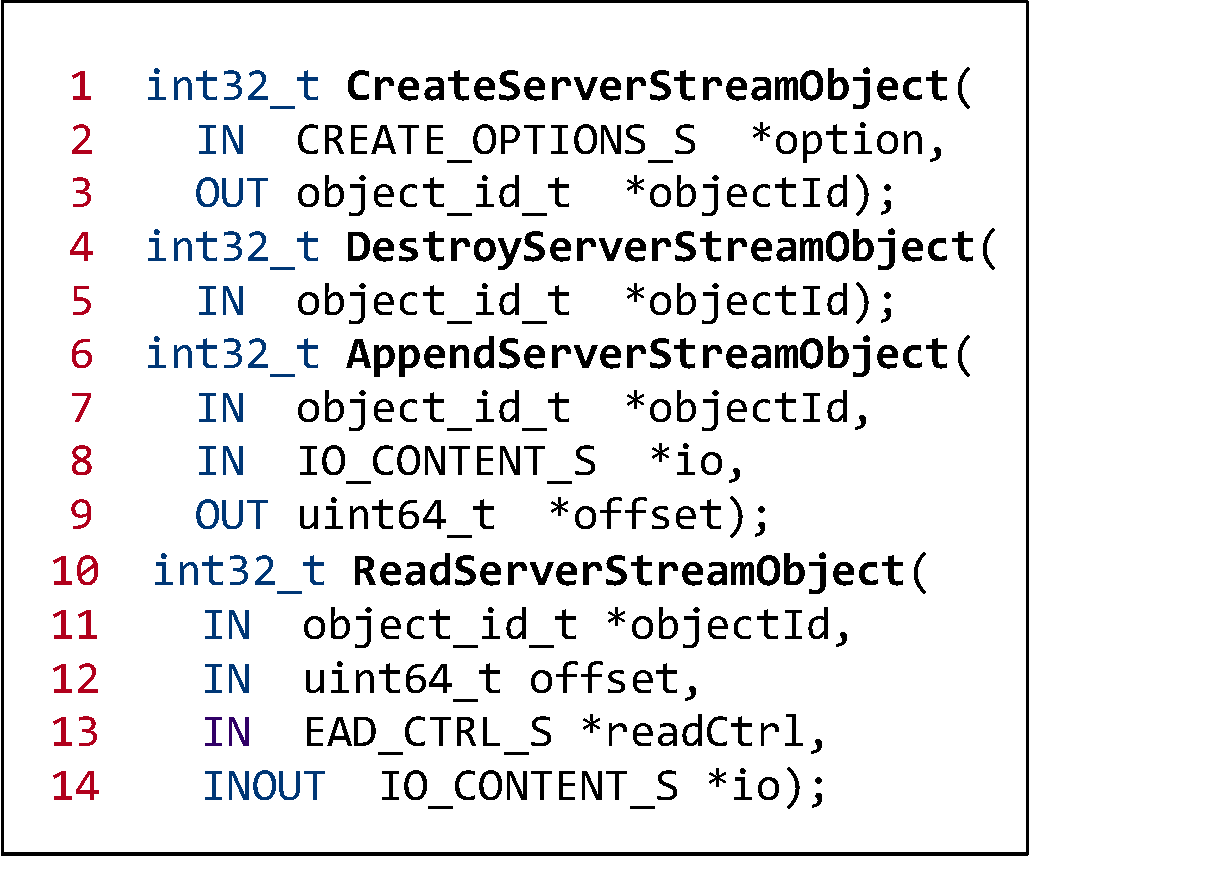
\includegraphics[scale=0.35]{figures/streamobject}
	\vspace{-1em}
	\caption{Stream Object Operations.}
	\label{fig:streamobject}
	\vspace{-2em}
\end{figure}



\noindent \textbf{Write stream messages.} We discuss how to write messages into \sys and endure enterprise-level load-balanced and redundant persistence for the stream objects, which is achieved on the basis of SSD and HDD storage pools.  As shown in Figure~\ref{fig:write}, the messages are first   assigned to stream object slices based on topics, keys, and offsets (Figure~\ref{fig:write}-a,b,c). Then, a distributed hash table is leveraged to ensure even data distribution for load-balance storage (Figure~\ref{fig:write}-d). Specifically, data slices will be distributed evenly to 4096 logical shards, each of which has the storage space managed by persistence logs (PLog, Figure~\ref{fig:write}-e). Each PLog unit is a collection of persistence services in OceanStor~\cite{huawei} that controls a fixed amount of storage space on multiple disks and provides 128 MB of addresses per shard. When a message is received, the PLog unit replicates it to multiple disks for redundancy (Figure~\ref{fig:write}-f). We use  key-value databases to serve as indexes for PLogs for fast record lookup.


\begin{figure}[htbp]	
	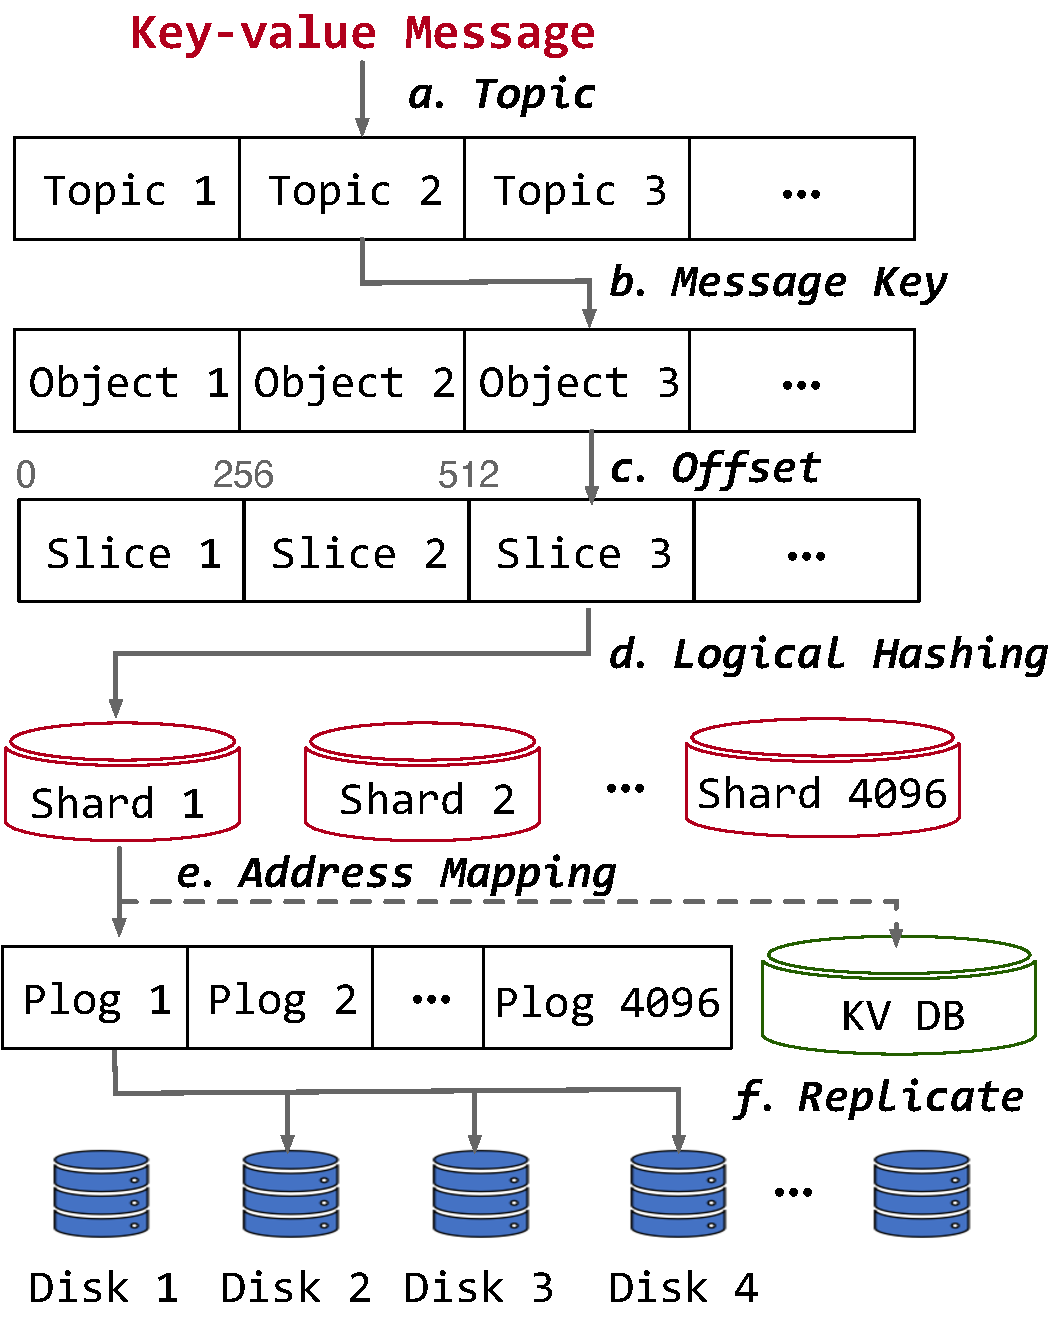
\includegraphics[scale=0.3]{figures/write}
	\centering
	\vspace{-1em}
	\caption{Write Message to \sys.}
	\label{fig:write}
	\vspace{-1em}
\end{figure}


\subsection{Table Object}~\label{subsec:tableobject}
We also extend the storage object layer in \sys to support operations over tables for more effective data storage and management, like the lakehouse systems~\cite{iceberg,hudi,delta}. The table storage uses an open lakehouse format with putting catalog in KV store  for faster metadata access. The table abstraction is logically defined by a directory of data and metadata files, as shown an example  in Figure~\ref{fig:tableobject}.

\noindent \textbf{\texttt{Data} directory.} Table objects are stored in Parquet files of the \texttt{data} directory. In this example, the table is partitioned based on the date column, so the data objects are separated into different sub-directories by the location. Each sub-directory name represents its partition range. The data objects in each Parquet file are organized as row-groups and stored in a columnar format for efficient data analysis. Footers in the Parquet files contain statistics to support data skipping within the file.




\noindent \textbf{\texttt{Metadata} directory}  keeps track of the file paths of the table, table schema,  and transaction commits etc., which are organized into three levels: commit, snapshot, and catalog, as shown in Figure~\ref{fig:tableobject}-(b, c, d).

 \noindent \underline{\textit{Commits}} are \texttt{Arvo} files that contain file-level metadata and statistics such as file paths, record counts, and value ranges for the data objects. Each data insert, update, and delete operation will generate a new commit file to record changes of the data object files.


\noindent \underline{\textit{Snapshots}} are index files that index  valid commit files for a specified time period. These snapshots document commit statistics such as current files, row count and added/removed files/rows as data operation logs. Along with commits, snapshots provide snapshot-level isolation to support optimistic concurrency control. Readers can access the data by reading from the valid commit files, while changes made by a writer will not be visible to readers until they are committed and recorded in a snapshot. This allows for multiple readers and one writer to access the data simultaneously without the need for locks. 

Snapshots also monitor the expiration of all commits, making them essential for supporting time travel. Time travel queries allow data to be viewed as it appeared at a specific time. By keeping old commits and snapshots, the table object enables the use of a timestamp to look up the corresponding snapshot and commits, so as to access to historical data.

\noindent \underline{\textit{Catalog}}  describes the table object, including the profile data  such as the table ID, directory paths, schema, snapshot descriptions, modification timestamps, etc. The data and metadata files are stored in the table directory, except for the catalog, which is stored in a distributed key-value engine optimized for RDMA and SCM to ensure fast metadata access. The data and metadata files are converted to PLogs in the underlying storage for redundant persistence as discussed above.



\begin{figure}[htbp]
	
	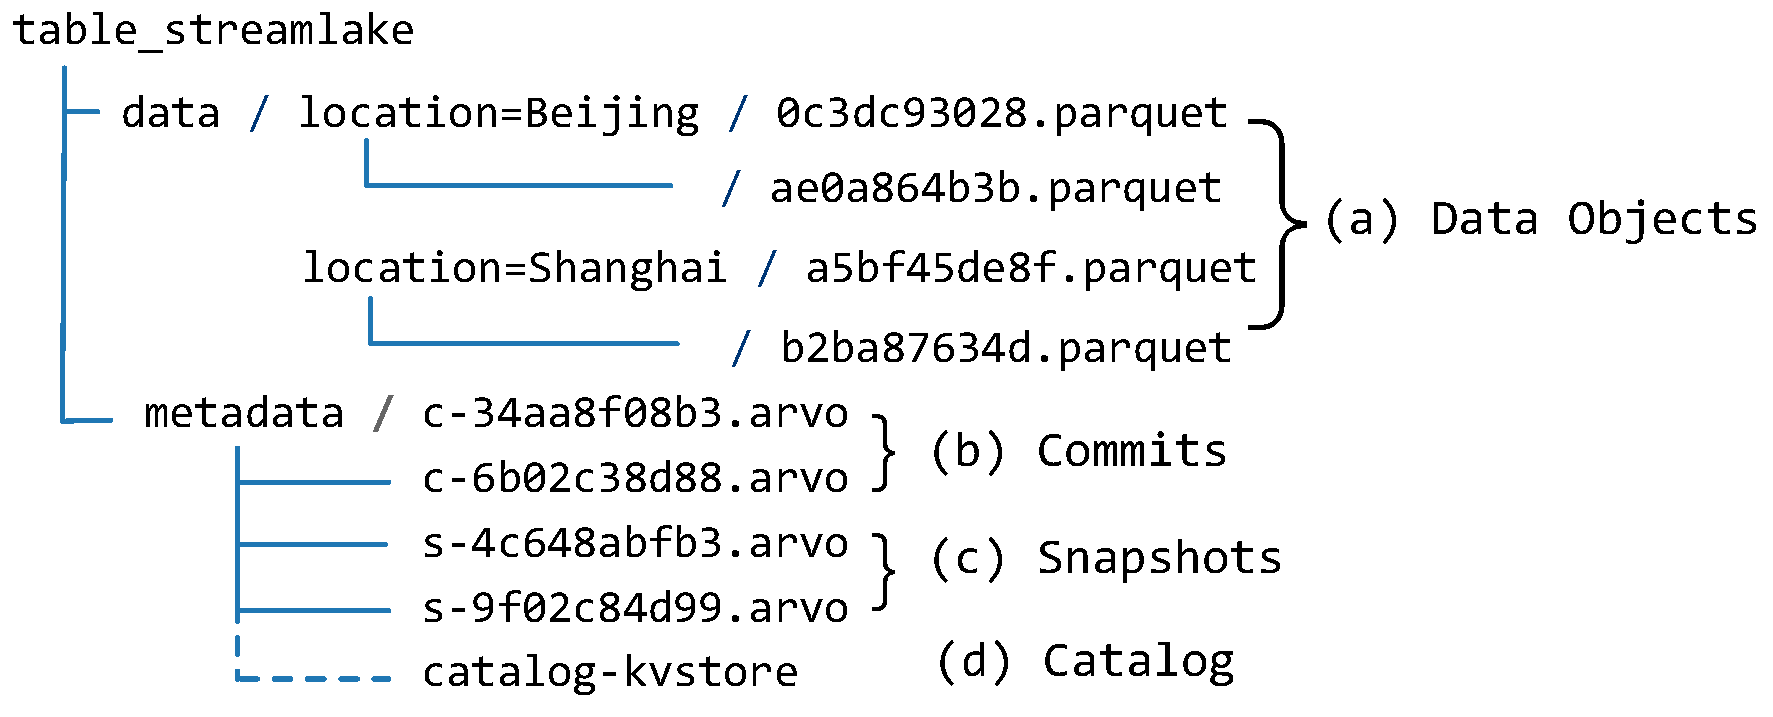
\includegraphics[scale=0.3]{figures/tableobjects}
	\centering
	\vspace{-1em}
	\caption{File Organization of \sys Table Objects.}
	\label{fig:tableobject}
	\vspace{-1em}
\end{figure}


















